%===============================================================================
% LaTeX sjabloon voor de bachelorproef toegepaste informatica aan HOGENT
% Meer info op https://github.com/HoGentTIN/bachproef-latex-sjabloon
%===============================================================================

\documentclass{bachproef-tin}

\usepackage{hogent-thesis-titlepage} % Titelpagina conform aan HOGENT huisstijl

%%---------- Documenteigenschappen ---------------------------------------------
% TODO: Vul dit aan met je eigen info:

% De titel van het rapport/bachelorproef
\title{Onderzoek naar samenwerking tussen Cloud-Init en Ansible}

% Je eigen naam
\author{Maarten De Smedt}

% De naam van je promotor (lector van de opleiding)
\promotor{Lotte Van Steenberghe}

% De naam van je co-promotor. Als je promotor ook je opdrachtgever is en je
% dus ook inhoudelijk begeleidt (en enkel dan!), mag je dit leeg laten.
\copromotor{Simon Lepla}

% Indien je bachelorproef in opdracht van/in samenwerking met een bedrijf of
% externe organisatie geschreven is, geef je hier de naam. Zoniet laat je dit
% zoals het is.
\instelling{Be-Mobile}

% Academiejaar
\academiejaar{2018-2019}

% Examenperiode
%  - 1e semester = 1e examenperiode => 1
%  - 2e semester = 2e examenperiode => 2
%  - tweede zit  = 3e examenperiode => 3
\examenperiode{2}

%===============================================================================
% Inhoud document
%===============================================================================

\begin{document}

%---------- Taalselectie -------------------------------------------------------
% Als je je bachelorproef in het Engels schrijft, haal dan onderstaande regel
% uit commentaar. Let op: de tekst op de voorkaft blijft in het Nederlands, en
% dat is ook de bedoeling!

%\selectlanguage{english}

%---------- Titelblad ----------------------------------------------------------
\inserttitlepage

%---------- Samenvatting, voorwoord --------------------------------------------
\usechapterimagefalse
%%=============================================================================
%% Voorwoord
%%=============================================================================

\chapter*{\IfLanguageName{dutch}{Woord vooraf}{Preface}}
\label{ch:voorwoord}

%% TODO:
%% Het voorwoord is het enige deel van de bachelorproef waar je vanuit je
%% eigen standpunt (``ik-vorm'') mag schrijven. Je kan hier bv. motiveren
%% waarom jij het onderwerp wil bespreken.
%% Vergeet ook niet te bedanken wie je geholpen/gesteund/... heeft

Maken als bachelorproef helemaal gedaan is.
%%=============================================================================
%% Samenvatting
%%=============================================================================

% TODO: De "abstract" of samenvatting is een kernachtige (~ 1 blz. voor een
% thesis) synthese van het document.
%
% Deze aspecten moeten zeker aan bod komen:
% - Context: waarom is dit werk belangrijk?
% - Nood: waarom moest dit onderzocht worden?
% - Taak: wat heb je precies gedaan?
% - Object: wat staat in dit document geschreven?
% - Resultaat: wat was het resultaat?
% - Conclusie: wat is/zijn de belangrijkste conclusie(s)?
% - Perspectief: blijven er nog vragen open die in de toekomst nog kunnen
%    onderzocht worden? Wat is een mogelijk vervolg voor jouw onderzoek?
%
% LET OP! Een samenvatting is GEEN voorwoord!

%%---------- Nederlandse samenvatting -----------------------------------------
%
% TODO: Als je je bachelorproef in het Engels schrijft, moet je eerst een
% Nederlandse samenvatting invoegen. Haal daarvoor onderstaande code uit
% commentaar.
% Wie zijn bachelorproef in het Nederlands schrijft, kan dit negeren, de inhoud
% wordt niet in het document ingevoegd.

\IfLanguageName{english}{%
\selectlanguage{dutch}
\chapter*{Samenvatting}
\lipsum[1-4]
\selectlanguage{english}
}{}

%%---------- Samenvatting -----------------------------------------------------
% De samenvatting in de hoofdtaal van het document

\chapter*{\IfLanguageName{dutch}{Samenvatting}{Abstract}}

Maken als bachelorproef klaar is.

\lipsum[1-4]


%---------- Inhoudstafel -------------------------------------------------------
\pagestyle{empty} % Geen hoofding
\tableofcontents  % Voeg de inhoudstafel toe
\cleardoublepage  % Zorg dat volgende hoofstuk op een oneven pagina begint
\pagestyle{fancy} % Zet hoofding opnieuw aan

%---------- Lijst figuren, afkortingen, ... ------------------------------------

% Indien gewenst kan je hier een lijst van figuren/tabellen opgeven. Geef in
% dat geval je figuren/tabellen altijd een korte beschrijving:
%
%  \caption[korte beschrijving]{uitgebreide beschrijving}
%
% De korte beschrijving wordt gebruikt voor deze lijst, de uitgebreide staat bij
% de figuur of tabel zelf.

\listoffigures
\listoftables

% Als je een lijst van afkortingen of termen wil toevoegen, dan hoort die
% hier thuis. Gebruik bijvoorbeeld de ``glossaries'' package.
% https://www.overleaf.com/learn/latex/Glossaries

%---------- Kern ---------------------------------------------------------------

% De eerste hoofdstukken van een bachelorproef zijn meestal een inleiding op
% het onderwerp, literatuurstudie en verantwoording methodologie.
% Aarzel niet om een meer beschrijvende titel aan deze hoofstukken te geven of
% om bijvoorbeeld de inleiding en/of stand van zaken over meerdere hoofdstukken
% te verspreiden!

%%=============================================================================
%% Inleiding
%%=============================================================================

\chapter{\IfLanguageName{dutch}{Inleiding}{Introduction}}
\label{ch:inleiding}
In dit hoofdstuk wordt er een kort inleiding over de bachelorproef. De oorsprong van het idee en de onderzoeksvraag wordt besproken. Ook wordt er al wat basisinfo gegeven over het onderwerp.


De installatie en modificatie van software servers moet voor de gebruiker altijd makkelijker en sneller. Eens de gebruiker weet wat voor server hij wil, wil hij deze liefst zo snel mogelijk opzetten met de nodige specificaties. Of als de gebruiker een kleine aanpassing wil doen aan de server, wil hij dit zo makkelijk mogelijk aanpassen. 

Om dit zo efficiënt mogelijk te doen heb je configuration management tools nodig. Dit zijn tools die gemaakt zijn om software op servers te installeren en te beheren. De meest bekende tools zijn Chef, Puppet, Salt en Ansible. In deze bachelorproef gaat het onder andere over Ansible. 

%De inleiding moet de lezer net genoeg informatie verschaffen om het onderwerp te begrijpen en in te zien waarom de onderzoeksvraag de moeite waard is om te onderzoeken. In de inleiding ga je literatuurverwijzingen beperken, zodat de tekst vlot leesbaar blijft. Je kan de inleiding verder onderverdelen in secties als dit de tekst verduidelijkt. Zaken die aan bod kunnen komen in de inleiding~\autocite{Pollefliet2011}:

%\begin{itemize}
%  \item context, achtergrond
%  \item afbakenen van het onderwerp
 % \item verantwoording van het onderwerp, methodologie
 % \item probleemstelling
  %\item onderzoeksdoelstelling
  %\item onderzoeksvraag
  %\item \ldots
%\end{itemize}

\section{\IfLanguageName{dutch}{Context}{Problem Statement}}
\label{sec:context}

Ansible is op zich al een zeer goede configuration management tool, maar voor het bedrijf Be-Mobile nog niet goed genoeg. 

Be-Mobile is een Big Data verkeersbedrijf. Be-Mobile wil verkeer revolutioneren en de mobiliteits oplossingen voor morgen en vandaag creëren. Hun hoofdzetel ligt in Melle, bij Gent. 

Be-Mobile werkt met "Hetzner Cloud". Dit is hun cloud server provider. Met hetzner cloud heb je de optie om te verwijzen naar een cloudconfig file om je server te configureren. Het cloudconfig bestand is het configuratie  bestand van cloud-init. 

Cloud-init is net zoals een Ansible een soort van configuration management tool maar speciaal voor cloud servers. Door middel van paramaters in te vullen in dit bestand kan je jouw server configureren.
 

%Uit je probleemstelling moet duidelijk zijn dat je onderzoek een meerwaarde heeft voor een concrete doelgroep. De doelgroep moet goed gedefinieerd en afgelijnd zijn. Doelgroepen als ``bedrijven,'' ``KMO's,'' systeembeheerders, enz.~zijn nog te vaag. Als je een lijstje kan maken van de personen/organisaties die een meerwaarde zullen vinden in deze bachelorproef (dit is eigenlijk je steekproefkader), dan is dat een indicatie dat de doelgroep goed gedefinieerd is. Dit kan een enkel bedrijf zijn of zelfs één persoon (je co-promotor/opdrachtgever).

\section{\IfLanguageName{dutch}{Probleemstelling - Onderzoeksvraag}{Research question}}
\label{sec:probleemstellingonderzoeksvraag}

Het probleem is meteen heel duidelijk. Moet er worden overgestapt naar cloud-init in plaats van Ansible. In deze bachelorproef gaat dit worden onderzocht. Waar zijn Ansible en cloud-init verschillend, waar zijn ze hetzelfde en waar vullen ze mekaar aan. De echte onderzoeksvragen waar deze thesis een antwoord op hoopt te vinden is:

\begin{itemize}
    \item Is Ansible overbodig door het gebruikt van Cloud-init?
    \item Zijn Ansible en cloud-init compatibel?
    \item Op welke manier zijn ze compatibel of overbodig?
\end{itemize}



%Wees zo concreet mogelijk bij het formuleren van je onderzoeksvraag. Een onderzoeksvraag is trouwens iets waar nog niemand op dit moment een antwoord heeft (voor zover je kan nagaan). Het opzoeken van bestaande informatie (bv. ``welke tools bestaan er voor deze toepassing?'') is dus geen onderzoeksvraag. Je kan de onderzoeksvraag verder specifiëren in deelvragen. Bv.~als je onderzoek gaat over performantiemetingen, dan 

%\section{\IfLanguageName{dutch}{Onderzoeksdoelstelling}{Research objective}}
%\label{sec:onderzoeksdoelstelling}
%misschien doen
%Wat is het beoogde resultaat van je bachelorproef? Wat zijn de criteria voor succes? Beschrijf die zo concreet mogelijk. Gaat het bv. om een proof-of-concept, een prototype, een verslag met aanbevelingen, een vergelijkende studie, enz.

\section{\IfLanguageName{dutch}{Opzet van deze bachelorproef}{Structure of this bachelor thesis}}
\label{sec:opzet-bachelorproef}

% Het is gebruikelijk aan het einde van de inleiding een overzicht te
% geven van de opbouw van de rest van de tekst. Deze sectie bevat al een aanzet
% die je kan aanvullen/aanpassen in functie van je eigen tekst.

De rest van deze bachelorproef is als volgt opgebouwd:

In Hoofdstuk~\ref{ch:inleidingtotansibleencloudinit} wordt een inleding gegeven tot Ansible en cloud-init

In Hoofdstuk~\ref{ch:stand-van-zaken} wordt een overzicht gegeven van de stand van zaken binnen het onderzoeksdomein, op basis van een literatuurstudie.

In Hoofdstuk~\ref{ch:methodologie} wordt de methodologie toegelicht en worden de gebruikte onderzoekstechnieken besproken om een antwoord te kunnen formuleren op de onderzoeksvragen.

In Hoofdstuk~\ref{ch:testlokaal} worden lokale testomgevingen  opgezet doormiddel van Vagrant en Virtualbox.

In Hoofdstuk~\ref{ch:testhetzner} worden testomgevingen opgezet doormiddel van Hetzner Cloud.

In Hoofdstuk~\ref{ch:basisconf} worden er basisconfiguraties gedaan op alle servers (aanmaken users, package installeren,..)

In Hoofdstuk~\ref{ch:serverconf} worden er verschillende soorten servers(file, web, dhcp, ...) gemaakt met de testomgevingen.

In Hoofdstuk~\ref{ch:naopstarten} wordt er gekeken hoe je instellingen aanpast na het opstarten van de server.

In Hoofdstuk~\ref{ch:container} wordt gekeken de configurtie containers en clusters wordt ondersteunt.

In Hoofdstuk~\ref{ch:conclusie}, tenslotte, wordt de conclusie gegeven en een antwoord geformuleerd op de onderzoeksvragen. Daarbij wordt ook een aanzet gegeven voor toekomstig onderzoek binnen dit domein.
\chapter{\IfLanguageName{dutch}{Stand van zaken}{State of the art}}
\label{ch:stand-van-zaken}

% Tip: Begin elk hoofdstuk met een paragraaf inleiding die beschrijft hoe
% dit hoofdstuk past binnen het geheel van de bachelorproef. Geef in het
% bijzonder aan wat de link is met het vorige en volgende hoofdstuk.

% Pas na deze inleidende paragraaf komt de eerste sectiehoofding.

%Dit hoofdstuk bevat je literatuurstudie. De inhoud gaat verder op de inleiding, maar zal het onderwerp van de bachelorproef *diepgaand* uitspitten. De bedoeling is dat de lezer na lezing van dit hoofdstuk helemaal op de hoogte is van de huidige stand van zaken (state-of-the-art) in het onderzoeksdomein. Iemand die niet vertrouwd is met het onderwerp, weet nu voldoende om de rest van het verhaal te kunnen volgen, zonder dat die er nog andere informatie moet over opzoeken \autocite{Pollefliet2011}.

%Je verwijst bij elke bewering die je doet, vakterm die je introduceert, enz. naar je bronnen. In \LaTeX{} kan dat met het commando \texttt{$\backslash${textcite\{\}}} of \texttt{$\backslash${autocite\{\}}}. Als argument van het commando geef je de ``sleutel'' van een ``record'' in een bibliografische databank in het Bib\LaTeX{}-formaat (een tekstbestand). Als je expliciet naar de auteur verwijst in de zin, gebruik je \texttt{$\backslash${}textcite\{\}}.
%Soms wil je de auteur niet expliciet vernoemen, dan gebruik je \texttt{$\backslash${}autocite\{\}}. In de volgende paragraaf een voorbeeld van elk.

%\textcite{Knuth1998} schreef een van de standaardwerken over sorteer- en zoekalgoritmen. Experten zijn het erover eens dat cloud computing een interessante opportuniteit vormen, zowel voor gebruikers als voor dienstverleners op vlak van informatietechnologie~\autocite{Creeger2009}.

In dit hoofdstuk wordt de stand van zaken besproken van cloud-init en Ansible. Eerst wordt uitgelegd wat Ansible is, wat de eigenschappen zijn en hoe het precies werkt. Daarna wordt er net hetzelfde met cloud-init gedaan. Ten laatste wordt er ook een literatuurstudie uitgevoerd op gevonden van het bachelorproefvoorstel.

\section{Ansible}
Ansible is een open source IT configuration management en deployment tool. Ansible hun grote doel is om besturingssysteem configuratie en de implementatie van software allemaal onder 1 systeem. De informatie werd gevonden met behulp van het document \textit{Ansible In Depth} \autocite{ansibleid}.

Ansible staat bekend als een systeem dat makkelijk te leren is als IT administrator, ontwikkelaar of manager. Het probeert er voor te zorgen dat het makkelijk te verstaan is en makkelijk om zelf op te bouwen. Zodat nieuwe gebruikers dit makkelijk kunnen oppikken. Ze proberen uniek te zijn door dingen door val aanpassing mogelijk te geven aan gebruikers voor de expert-gebruikers. Maar toch net zo toegankelijk voor de nieuwe gebruiker.

\subsection{Architectuur}
Eén van de belangrijkste verschillen tussen Ansible en andere configuratie management tools, is zijn architectuur. Ansible gaat uit van het ``push'' model. Ook is er geen additionele software nodig om machines bruikbaar te maken voor Ansible. Het heeft geen extra gebruikers of referenties nodig om te draaien. Het gebruikt gewoon de informatie die de user meegeeft. Daarbij hoort ook dat Ansible geen administrator of sudo toegang nodig heeft. Ansible wordt standaard bestuurt door een remote computer.

Dit zorgt ervoor dat Ansible veiliger wordt. Door alleen de informatie die de gebruiker meegeeft te gebruiken. Iemand die wel toegang heeft tot de server kan maar niet tot te remote computer kan geen aanpassingen pushen.

\subsection{Playbook - Roles}
Ansible voert de automatisatie en deployment uit via playbooks. Dit zijn yaml bestanden die beschrijven hoe de automatisatie moet verlopen. 

Deze playbooks bevatten verschillende ``plays'' die de automatisatie definiëren over verschillende hosts. Deze hosts staan bekend als de inventory. Elke ``play'' bevat verschillende taken die één, verschillende of alle hosts moeten uitvoeren. Elke taak roept een Ansible module aan, een klein stukje code dat een specifieke taak uitvoert. Deze kan kunnen zeer simpel zijn, een bestand op een machine zetten of een specifieke package installeren. Maar ze kunnen ook complex zijn zoals een gehele CloudFormation opstarten in Amazon EC2.
\begin{figure}[!htb]
    \center{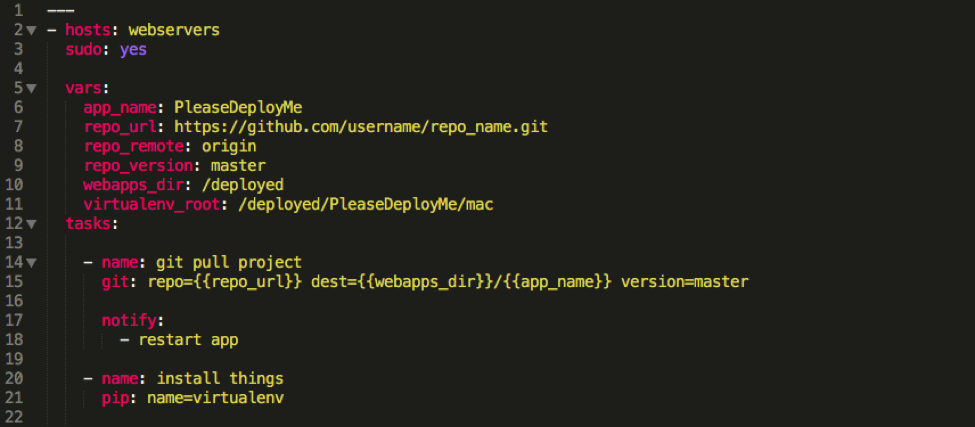
\includegraphics[width=0.9\textwidth]{img/playbookex.png}}
    \caption{Voorbeeld van een Ansible playbook.}
    \label{fig:playbook}
\end{figure}

Ansible is geschreven zodat als ze de playbook uitvoeren ook checken of deze task nog moet gedaan worden. Bijvoorbeeld als een Ansible taak is om een webserver op te starten, zal Ansible deze alleen uitvoeren als de webserver nog niet is opgestart. Dit staat bekend als idempotente. Het zorgt ervoor dat de configuratie altijd snel en efficiënt wordt uitgevoerd.

Met Ansible kunnen taken ook ingekapseld worden in een role. Dit wordt gebruikt als er een specifieke configuratie meerdere keren wordt uitgevoerd, bijvoorbeeld het opzetten van een webserver. De Ansible Galaxy site bevat veel roles die kunnen gebruikt en aangepast worden voor het gebruik in een playbook.
\begin{figure}[!htb]
    \center{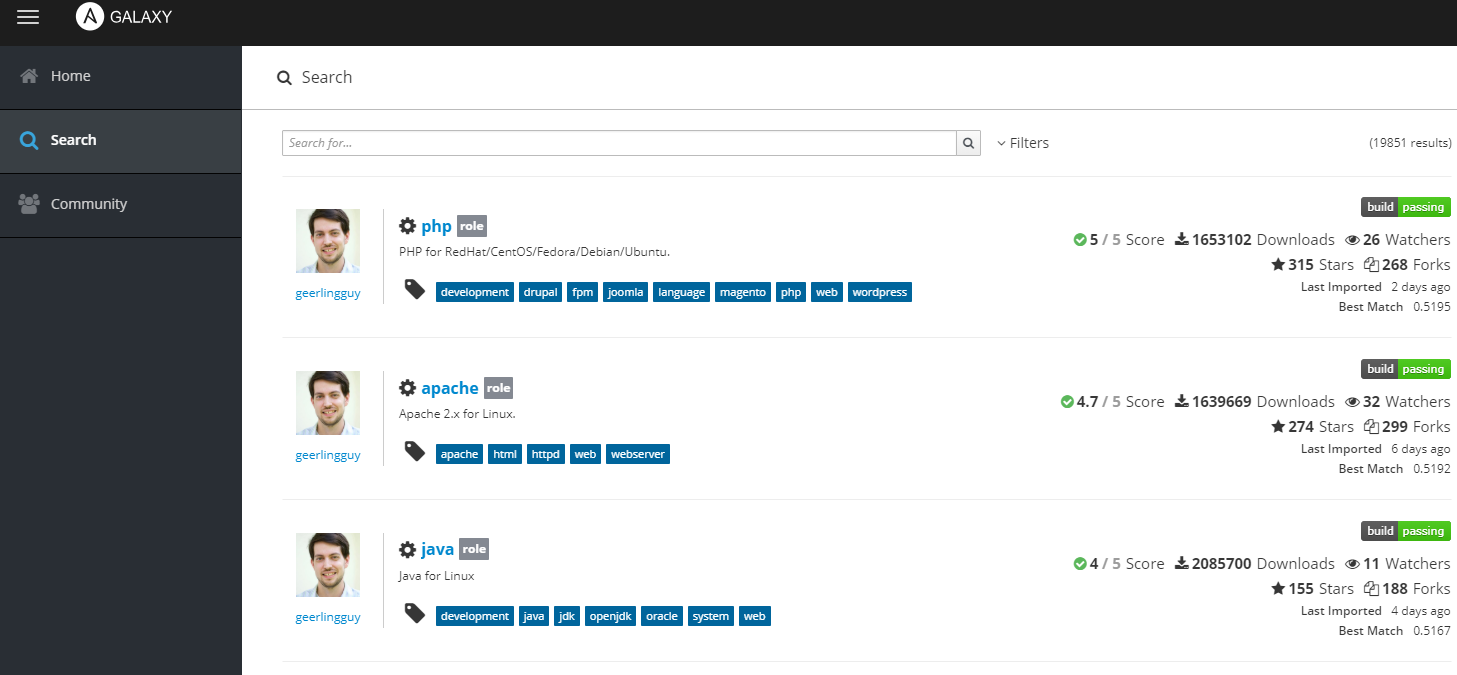
\includegraphics[width=0.9\textwidth]{img/agalaxy.png}}
    \caption{Ansible Galaxy site met lijst van roles.}
    \label{fig:agalaxy}
\end{figure}


\subsection{Omgevingen}
Ansible is even makkelijk te deployen in publieke of private cloud omgevingen, als in een lokale omgeving. Voor publieke of private cloud providers kan er gekozen worden voor: Amazon Web Services, Microsoft Azure, Rackspace,... Maar er kan ook op lokale infrastructuren gewerkt worden door middel van virtuele machines. Tools die hiervoor worden gebruikt zijn: VirtualBox, VMWare,...

\section{Cloud-Init}
Net als Ansible is cloud-init ook een soort van configuration manager en deployment tool. Het is geschreven in python. Cloud-init zorgt  voor de customisaties tijdens het opstarten van de cloud of virtuele instanties. Deze service gebeurt heel vroeg in het boot proces. De instantie zoekt naar de \textit{user data} (het cloud-init script) van de gebruiker en voert deze uit. De naam zegt het al zelf, maar cloud-init is een tool die meer wordt gebruikt door cloud instanties. Bijna alle cloud-providers hebben een functie waardoor er een cloud-init script kan meegeven worden. 

Veel van de punten die hier verder worden besproken zijn gevonden in de presentatie van \autocite{cloudred}.

\subsection{Modules}
Cloud-init heeft 6 hoofdpijlers waar het modules voor heeft, namelijk: schijf configuratie, commando's uitvoeren, gebruikers en groepen creeeren, beheren van packages, content bestanden schrijven en bootstrappen van Chef en/of Puppet. Er zijn nog andere modules maar dit zijn de 6 hoofdpijlers van cloud-init en daarbij de meeste gebruikte modules. Er kunnen ook zelf modules toevoegd worden door deze in Python te schrijven. Met behulp van de documentatie van \textcite{clouddocs} wordt er per pijler uitleg gegeven. 

\subsubsection{Schijf configuratie}
Er is 1 module die wordt gebruikt voor de schijf configuratie, namelijk \textbf{Disk Setup}. Via deze module kunnen er simpele paritities en bestandsystemen worden geconfigureerd. Via de \textit{device\_aliases} richtlijnen kunnen er aliassen worden gemaakt voor de de block devices. Zodat er makkelijker naar deze kan worden verwezen. Via de \textit{disk\_setup} richtlijn wordt de partitie configuratie gedaan. De \textit{table\_type} richtlijn wordt gebruikt om de partitie tabel mee te gegeven. Ten laatste is er ook de \textit{fs\_setup} richtlijn deze wordt gebruikt om de systeembestand configuratie te doen.

\subsubsection{Commando's uitvoeren}
Voor het uitvoeren van commando's zijn er 2 modules: \textbf{Runcmd} en \textbf{Bootcmd}. Beide bevatten maar 1 richtlijn namelijk \textit{runcmd} en \textit{bootcmd}. Bij \textit{runcmd} worden de command's die worden meegegeven elke keer uitgevoerd als het script wordt gedraaid. Bij \textit{bootcmd} enkel alleen als de instantie wordt opgestart. Ook worden de commando's bij \textit{bootcmd} veel vroeger in het bootproces uitgevoerd.

\subsubsection{Gebruikers en groepen}
Ook voor Gebruikers en groepen is er slechts 1 module: \textbf{Users and Groups}. Groepen kunnen worden toegevoegd door deze aan de richtlijn \textit{groups} toe te voegen samen eventuele configuratie per groep. Gebruikers kunnen dan weer toegevoegd worden door deze aan de richtlijn \textit{users} toe te voegen. Ook bij de gebruikers kan er nog extra configuratie gedaan worden per gebruiker.

\subsubsection{Packages}
Voor het beheren en configueren van packages zijn er verschillende modules: \textbf{Apt Configure}, \textbf{Apt Pipelining}, \textbf{Package Update Upgrade Install}, \textbf{Snap}, \textbf{Snappy} en \textbf{Yum Add Repo}. Er kunnen packages geïnstalleerd en geconfigureerd worden via Yum en Apt. Meestal ondersteund een besturingsysteem Yum of Apt. Voor installatie van een package moeten deze plaatsen bij de richtlijn \textit{packages}. Cloud-init weet zelf of het met yum of apt wordt gedaan. De configuratie en het toevoegen van package repo's gebeurt via Apt Configure, Apt Pipelinig en Yum Add Repo. Ook ondersteunt cloud-init de installatie van snap packages. Dit zijn gecontaineriseerde packages. Via Snappy kan deze geconfigureerd worden.

\subsubsection{Content bestanden}
Voor het aanmaken van bestanden is er de module \textbf{Write Files}. In de richtlijn \textit{write\_files} word de gecodeerde inhoud van het bestand gezet met het pad.

\subsubsection{Chef - Puppet}
Ook zijn er 2 modules die Chef en Puppet installeren, configureren en starten. Deze modules zijn logischer wijs \textbf{Chef} en \textbf{Puppet}. Voor Puppet wordt de richtlijn \textit{puppet} meegegeven. Daaronder worden alle configuraties geplaatst. Chef werkt op dezelfde manier.

\subsection{User Data - Cloud config}
Zoals Ansible zijn playbook heeft, heeft cloud-init zijn user data. Ook heeft cloud-init de meta-data, maar deze wordt meegegeven door het cloud platform zelf. Dit zijn bijvoorbeeld de server naam en het server id. De 2 bekendste methodes om user data mee te geven zijn User-Data Script en Cloud Config Data. 
\subsubsection{User-Data Script}
Het User-Data script een linux script dat de server overloopt voor dat hij opstart. Het moet alijd beginnen met \textit{!\#} of \textit{Content-Type: text/x-shellscript}. Als er echt wordt gebruikt gemaakt van cloud-init wordt deze methode niet gebruikt. De modules kun je via zo een script bijvoorbeeld niet aanroepen. Dit is eerder voor gebruikers die al een script hebben. In plaats van dit om te zetten naar Cloud Config Data, kunnen ze dat dan script gebruiken.
\begin{figure}[!htb]
	\center{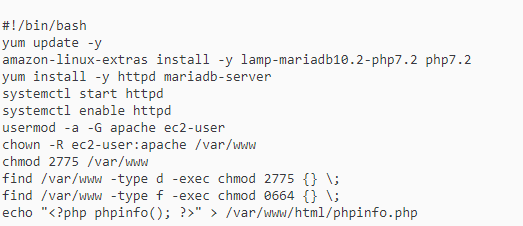
\includegraphics[width=0.9\textwidth]{img/userdatascript.png}}
	\caption{Voorbeeld user-data script.}
	\label{fig:udatascript}
\end{figure}

\subsubsection{Cloud Config Data}
De meest gebruikte methode is Cloud Config Data. Dit is een yaml bestand met de configuratie van de server in. Een Cloud Config bestand begint altijd met \textit{\#cloud-config}. In het bestand worden de modules opgelijst die worden gebruikt en daaronder dan hun configuraties. Dit bestand is veel overzichtelijker dan een script om later aan te passen of om te beheren. Ook heeft het wat gelijkenissen met het playbook van Ansible, doordat dit beide yaml bestanden zijn.
\begin{figure}[!htb]
	\center{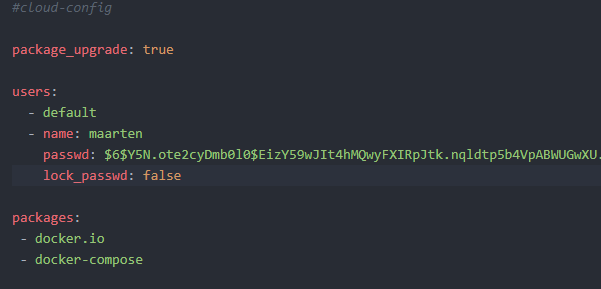
\includegraphics[width=0.9\textwidth]{img/cloudconfig.png}}
	\caption{Voorbeeld Cloud Config Data.}
	\label{fig:udatascript}
\end{figure}

\section{Studie 1}


%%=============================================================================
%% Methodologie
%%=============================================================================

\chapter{\IfLanguageName{dutch}{Methodologie}{Methodology}}
\label{ch:methodologie}

%% TODO: Hoe ben je te werk gegaan? Verdeel je onderzoek in grote fasen, en
%% licht in elke fase toe welke stappen je gevolgd hebt. Verantwoord waarom je
%% op deze manier te werk gegaan bent. Je moet kunnen aantonen dat je de best
%% mogelijke manier toegepast hebt om een antwoord te vinden op de
%% onderzoeksvraag.
In dit hoofdstuk wordt besproken welke methodes er gehanteerd zijn om de resultaten te bekomen. Dit hoofdstuk is onderverdeeld in 2 delen. Ten eerste wordt er info gegeven over de 2 testomgevingen. Ten tweede wordt er besproken welke testcriteria er gekozen zijn en waarom. In deze bachelorproef wordt er vooral focus gelegd op het de praktijk, het is een praktische onderzoek.

\section{Testomgevingen}
Voor het onderzoek moeten er verschillende testomgevingen worden opgesteld, om alles in te testen. Er is een lokale virtueel  omgeving en een omgeving op cloud servers. Er is gekozen voor deze twee omgevingen omdat dit de 2 meest voorkomende omgevingen zijn in de praktijk bij server management tools. 

Ansible is al een tool die gebruikt wordt voor virtuele omgevingen door gebruikers thuis, maar ook in grote cloud omgevingen voor bedrijven. Het zou dus niet correct zijn om het alleen lokaal te testen of alleen op de cloud. 

Voor het onderzoek is dit ook interessant want er is veel meer kans op verschillende resultaten. Die kunnen dan met elkaar worden vergeleken en dan kan er worden bekeken wat de oorzaak hiervan is. Dit geeft ook een mogelijkheid om het onderzoek in de toekomst verder te onderzoeken. Waarom bijvoorbeeld Ansible beter is lokaal zonder cloud-init dan met (dit is een hypothetische stelling).

\newpage
Per omgeving is er hieronder wat meer informatie te vinden. Over het opzetten van de omgevingen zijn voor beide aparte hoofdstukken aan toegewijd, namelijk: Hoofdstuk \ref*{ch:testlokaal} en Hoofdstuk \ref*{ch:testhetzner}.

\subsection{Lokaal}
Voor de lokale omgeving zal er worden gewerkt met 2 technologieën, namelijk: VirtualBox en vagrant. 

VirtualBox is een programma waarmee je virtuele machines kunt aanmaken en beheren. Hiermee worden de servers lokaal aangemaakt. 

Het tweede programma dat wordt gebruikt is vagrant. Vagrant is een command tool die die servers configureerd. In de actieve directory wordt het commando \textit{vagrant init} gedaan, dan staat er een \textit{vagrantfile}. Dit is het bestand dat kan worden geconfigureerd naargelang de wens van de gebruiker. Daarna wordt het commando \textit{vagrant up} gedaan. Dit start de server op. De server wordt opgestart met behulp van een tool die virtuele machines beheert en aanmaakt. In dit geval dus VirtualBox.
\begin{figure}[!htb]
	\center{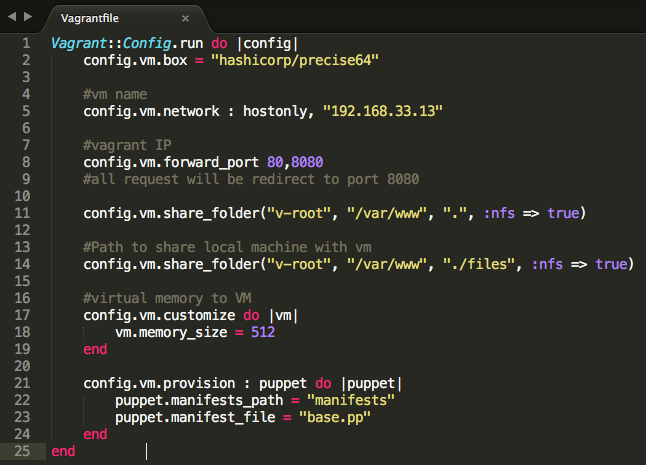
\includegraphics[width=0.9\textwidth]{img/vagrantexamp.png}}
	\caption{Voorbeeld van een vagrantfile.}
	\label{fig:vagrantexamp}
\end{figure}

\newpage
\subsubsection{Laptop}
Deze testomgeving wordt opgezet op de laptop: \textbf{Asus X750L}. Asus bracht deze laptop eind 2013 op de markt. De laptop is aangekocht in augustus 2014, en is bij het uitvoeren van het onderzoek bijna 5 jaar oud. Bijna alle specificaties zijn hetzelfde toen hij werd aangekocht. Alleen is de harde schijf vervangen van een HDD van 500 gigabyte naar een SSD van 500 gigabyte. Deze vervanging werd begin 2019 gedaan en bij het uit voeren van het onderzoek is dat 2-3 maand geleden. Hieronder is een  uitgebreide tabel met specificaties van de laptop. De data is verkregen door: \autocite{asuslaptop}.

\begin{table}
	\centering
	\begin{tabular}{c l}
		\hline
		\multicolumn{2}{c}{\textbf{Specificaties}} \\
		\hline
		Fabrikant & Asus \\
		\hline
		Model & ASUS x750L \\
		\hline		
        Besturingssysteem & Windows 10\\
        \hline
		CPU & Intel Core i7 4500U @ 2.4 GHz  \\
		\hline
		Geheugen & 8GB DDR3 @ 1600MHz \\
		\hline
		GPU & Nvidia GeForce GT 740M \\
		\hline
		Interne schijven & Crucial MX500 (500 GB) \\
		\hline
	\end{tabular}
	\caption{Specificaties van de laptop.}
	\label{tab:specs_desktop }
\end{table}

\begin{figure}[!htb]
	\center{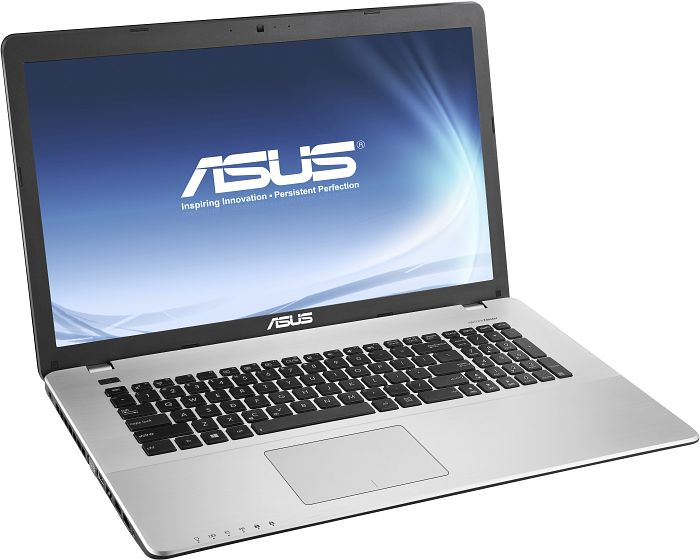
\includegraphics[width=0.4\textwidth]{img/testpcasus.jpg}}
	\caption{Foto van de laptop.}
	\label{fig:asustest}
\end{figure}

\subsection{Cloud}
Voor de cloud omgeving wordt er Hetzner Cloud gebruikt. In de inleiding is het bedrijf Be-Mobile al vernoemd en werd ook al gezegd dat zijn één van de redenen van het onderzoek zijn. Via hun is er toegang verkregen op een Hetzner Cloud omgeving om in te testen. 

Hetzner is een Duits bedrijf dat gespecialiseerd is in het hosten van servers. Hun datacenters liggen in Nuremberg (Duitsland), Falksenstein (Duitsland) en Helsinki (Finland). 

Via de commandline tool werden de server aangemaakt. Ook wordt er een SSH sleutel voorzien zodat er toegang is tot de aangemaakte servers. Info van hetzner werd gevonden dankzij de site van \autocite{hetzner}.


\section{Testcriteria}
Het volgende dat wordt besproken is de keuze van de testcriteria die werd gekozen in hoofdstukken~\ref{ch:basisconf},~\ref{ch:serverconf},~\ref{ch:naopstarten} en~\ref{ch:container}. 

In Hoofdstuk \ref*{ch:basisconf} worden basis configuraties op de server uit gevoerd. Dit om te bekijken wat de beste optie is om te kiezen als er gewoon wat kleine basis configuraties worden veranderd. Dit kan gebruikers aanmaken zijn, maar ook: commando's uitvoeren, mappen aanmaken. 

In Hoofdstuk \ref*{ch:serverconf} worden verschillende servers geïnstalleerd. Zo wordt er bekeken of het installeren en configureren van servers een ander resultaat heeft dan basis configuraties. Ook om te bekijken of er verschillen zijn per server.

In Hoofdstuk \ref*{ch:naopstarten} gaat er worden gekeken met welke optie je de server best aanpast na het opstarten. Als de server al opgestart is maar er wordt een klein dingetje verandert in het script. Welke optie is dan het best om snel deze verandering door te voeren.

Ten laatste wordt er in Hoofdstuk \ref*{ch:container} gekeken naar de configuratie van containers en clusters. Bijna elk bedrijf gebruikt containers en clusters voor hun netwerk. Het is dus logisch om te bekijken wat hier de resultaten zijn. Misschien zijn deze wel helemaal anders dan de resultaten van hiervoor.

\glossary{test}
%% Basis Configuratie, sever inst en conf, instellingen aanpassen na opstarten en container/cluster.



% Voeg hier je eigen hoofdstukken toe die de ``corpus'' van je bachelorproef
% vormen. De structuur en titels hangen af van je eigen onderzoek. Je kan bv.
% elke fase in je onderzoek in een apart hoofdstuk bespreken.

%\input{...}
%\input{...}
%...
\chapter{\IfLanguageName{dutch}{Opzetten lokale testomgeving}{Introduction}}
\label{ch:testlokaal}

In dit hoofstuk wordt besproken hoe de lokale testomgevingen zijn opgezet. Er zijn 3 lokale testomgevingen. De eerste is één die cloud-init gebruikt, de tweede gebruikt Ansible en de derde gebruikt cloud-init en Anisble. Voor het opzetten wordt er VirtualBox en Vagrant gebruikt.

\section{Cloud-init}
De eerste testomgeving die wordt besproken is die met cloud-init. Hij werd opgezet met behulp van: \autocite{cloudVagrant}. Er wordt hiervoor in 2 stappen gewerkt. Eerst wordt er een ISO met de cloud-init configuraties aangemaakt met behulp van de setup van \autocite{cloudVagrant}. Erna wordt deze ISO toegevoegd aan de testomgeving.

\subsection{Maken van ISO}
Voor het aanmaken van de ISO is er een Linux omgeving nodig. Allereest wordt er een omgeving opgezet om de ISO's in te maken. Deze wordt ook opgezet met Vagrant en VirtualBox. De box \textit{ubuntu/xenial64} wordt gebruikt (dit is dezelfde als degene die later in de testomgeving wordt gebruikt). Met het commando \textit{vagrant up} wordt de server aangemaakt. De vagrantfile ziet er zo uit:
\begin{lstlisting}
Vagrant.configure(''2'') do |config|
	config.vm.box =''ubuntu/xenial64''
end
\end{lstlisting}

Via het commando \textit{vagrant ssh} hebben we de toegang tot de server. Eens die er is tot de machine, wordt de package \textit{genisoimage} geïnstalleerd. Dit wordt via het commando \textit{sudo apt-get install genisoimage}. 

Nadat die package geïnstalleerd is wordt er een user-data bestand aangemaakt. In dit bestand komt de cloudconfig data. Hierna wordt een tweede bestand aangemaakt, namelijk het meta-data bestand. In dit bestand komt er nog extra minimale configuratie. De local-hostname en instance-id moeten hierin worden gezet.

Als deze bestanden zijn aangemaakt wordt er een Makefile gecreeërd. Via dit bestand wordt de iso aangmaakt. Zo ziet de Makefile eruit:
\begin{lstlisting}
nocloud.iso: meta-data user-data
    mkisofs \
        -joliet -rock \
        -volid "cidata" \
        -output nocloud.iso meta-data user-data
\end{lstlisting}

Ten laatste wordt het \textit{make} package geïnstalleerd. Via het commando \textit{make} wordt het iso bestand aangemaakt.

\subsection{Opzetten van testomgeving met cloud-init configuraties}
Er wordt een tweede omgeving aangemaakt (de effectieve testomeving) weer doormiddel van Vagrant en VirtualBox. Net zoals in het vorige gedeelte wordt ook hier de box \textit{ubuntu/xenial64} gebruikt.

In het vorige gedeelte is het iso bestand aangemaakt met de cloud-init configuraties. Allereerst moet dit iso bestand worden gekopieerd naar de map van de omgeving. In de vagrantfile die wordt gebruikt moet er dan worden doorverwezen deze iso. Dit wordt gedaan met deze configuraties in de vagrantfile.
\begin{lstlisting}
IMAGE_PATH = File.join(File.dirname(__FILE__), "no-cloud.iso")

Vagrant.configure(2) do |config|
	
    config.vm.box = "ubuntu/xenial64"
	
    config.ssh.password = nil	
    config.vm.synced_folder ".", "/vagrant", disabled: true
	
    config.vm.provider :virtualbox do |vb|
	  vb.customize [
	    "storageattach", :id,
	    "--storagectl", "SCSI",
	    "--port", "1",
	    "--type", "dvddrive",
	    "--medium", IMAGE_PATH
	]
	vb.linked_clone = true
   end
end
\end{lstlisting}
Als hierna \textit{vagrant up} wordt gedaan, wordt de server aangemaakt met de configuraties van cloud-init.
 
\section{Ansible}
De tweede lokale testomgeving die wordt opgezet is die met Ansible. Deze is niet zo complex om op te zetten als degene met cloud-init. Deze wordt opgezet met behulp van \autocite{ansibleVagrant}. Ook deze omgeving gebruikt Vagrant en VirtualBox. Als box wordt ook weer dezelfde gebruikt als de vorige keren. 

Er zijn eigenlijk maar 2 stappen die moeten worden gedaan. Allereest moet er een playbook bestand worden aangemaakt. Deze moet ook aanwezig in de locatie van de omgeving. De tweede stap is verwijzen naar dit playbook via de vagrantfile. Dit wordt op deze manier gedaan.
\begin{lstlisting}
Vagrant.configure(2) do |config|
    config.vm.box = "ubuntu/xenial64"
    
    config.vm.provision "ansible" do |ansible|
      ansible.verbose = "v"
      ansible.playbook = "playbook.yml"
   end
end
\end{lstlisting}

\section{Cloud-init \& Ansible }
to do
\chapter{\IfLanguageName{dutch}{Opzetten Hetzner Cloud testomgeving}{Introduction}}
\label{ch:testhetzner}
In dit hoofdstuk wordt besproken hoe de testomgevingen met Hetzner zijn opgezet. Er zijn 3 omgevingen: één met cloud-init, één met Ansible en één met cloud-init en Ansible.

\section{Aanmaken server met Hetzner}
Het aanmaken van servers kan op verschillende manieren. Hier wordt er gekozen om dit te doen via de command line. Via de site van Hetzner kan je hun command tool downloaden. Via het commando \textbf{hcloud} kunnen er nu server worden aangemaakt en beheert. Voor toegang te krijgen tot Hetzner Cloud moet je een bepaald bedrag betalen. Hierna kan je netwerken opzetten en via een Hetzner Token kan je op dit netwerk servers toevoegen. Via het bedrijf Be-Mobile is er toegang tot een Hetzner Cloud netwerk, met daarvoor een Hetzner Token.

Voor het aanmaken van de server zijn er 2 variabelen die worden toegevoegd. \textbf{Name}, de naam van de server, zo kunnen de servers uit elkaar houden. \textbf{Ssh-key}, via Hetzner kan je een ssh sleutel toevoegen om toegang te verkrijgen op de server. Via het bedrijf Be-Mobile is er een ssh sleutel verkegen. Het commando  voor het aanmaken van een server is dan:
\begin{lstlisting}[basicstyle=\small]
hcloud server create --name <naam van de server> 
    --ssh-key <naam van de sleutel in hetzner>
\end{lstlisting}
\newpage
Er zijn nog twee andere belangerijke commando's die worden gebruikt. Via het commando hieronder is er een lijst met alle servers die beschikbaar zijn.
\begin{lstlisting}[basicstyle=\small]
hcloud server list
\end{lstlisting}
Het commando hieronder verwijdert een server.
\begin{lstlisting}[basicstyle=\small]
hcloud server delete <naam of id van de server>
\end{lstlisting}


\section{Cloud-init}
Het opzetten van een omgeving met cloud-init in Hetzner Cloud is eigenlijk zeer simpel. Op \autocite{hetznerWiki} staat  dat bij het maken van de server \textit{user data} kan worden toegevoegd. Zoals werd gezien in hoofdstuk ~\ref{ch:cloud-init} is dit de data die cloud-init gebruikt voor zijn configuraties.

De user data is een vairbale die moet worden toegevoegd zoals de naam een ssh sleutel. Via \textbf{user-data-from-file} kan er een bestand worden toegevoegd tijdens het aanmaken van de server met de user data. Het commando dat wordt gebruikt om een server aan te maken ziet er dan zo uit:
\begin{lstlisting}[basicstyle=\small]
hcloud server create --name <naam van de server> 
    --ssh-key <naam van de sleutel in hetzner>
    --user-data-from-file <pad naar bestand>
\end{lstlisting}

\section{Ansible}
Het opzetten van een omgeving in Hetzner Cloud met Ansible is niet zo makkelijk. Er is geen variabale \textit{playbook} beschikbaar waar er een Ansible playbook kan aan worden toegevoegd.

Er zal gewerkt worden met behulp van GitHub. Het playbook dat wordt uitgevoerd, zal worden verkregen met een \textit{git clone} of \textit{git pull}. Daarna zal het worden uitgevoerd aan de hand van het commando:
\begin{lstlisting}[basicstyle=\small]
ansible-playbook -i, <playbook bestand>
\end{lstlisting}
Via dit commando wordt het playbook op de localhost uitgevoerd. 



\newpage
\section{Ansible \& cloud-init}
Het opzetten van een omgeving met Ansible en cloud-init wordt gedaan door een combinatie van de vorige 2 manieren. De server wordt opgezet met het commando:
\begin{lstlisting}[basicstyle=\small]
hcloud server create --name <naam van de server> 
--ssh-key <naam van de sleutel in hetzner>
--user-data-from-file <pad naar bestand>
\end{lstlisting}
De commando's die worden uitgevoerd om een Ansible playbook uit te voeren, worden in cloud-init verwerkt. In de module \textit{runcmd} wordt eerst het commando \textit{git clone} gezet, met verwijzing naar de repo met het playbook. Erna wordt het commando \textit{ansible-playbook} er gezet, deze voert het playbook uit.

Het enige extra dat wordt toegevoegd is een private ssh sleutel. Dit is de ssh-sleutel die toelaat dat je de git repo mag binnenhalen. Deze voegen we toe doormiddel van de module \textit{ssh\_keys} en daar de submodule \textit{rsa\_private}. Er worden ook nog 2 commando's boven de andere 2 geplaatst zodat dit werkt. Allereerst het commando \textit{ssh-keyscan github.com >> /etc/ssh/ssh\_known\_hosts}. Hiermee kent het systeem github en gaat dit geen error geven. Het tweede commando is \textit{ssh-agent bash -c 'ssh-add /etc/ssh/ssh\_host\_rsa\_key; git clone <repo>'}. Met dit commando zal cloud-init de ssh sleutel gebruiken die is toegevoegd.

\chapter{\IfLanguageName{dutch}{Basisconfiguraties op de servers}{Introduction}}
\label{ch:basisconf}
In dit hoofdstuk wordt voor het eerst een onderzoek uitgevoerd. 

Er wordt voor elke server een configuratie bestand gemaakt dat 4 basisconfiguraties zal uitvoeren: gebruikers en groepen toevoegen, packages installeren en updates, mappen structuur aanmaken en ssh configuratie. 


\section{Aanmaken configuratie bestanden}
In dit hoofdstuk zal uitglegd worden hoe de playbooks en cloudconfig bestanden worden aangemaakt en opgesteld. 

Eerst wordt uitgelegd hoe de cloud-init configuraties worden gedaan, erna het Ansible playbook. Ten laatste zullen de set-ups worden gemaakt waar een combinatie wordt gebruikt.

De gebruiker die zal worden aangemaakt is \textit{bachelor} met wachtwoord \textit{proef}. De gebruiker zal behoren tot de groep \textit{test} die ook zal worden aangemaakt. De packages die zullen worden geïnstalleerd zijn: \textit{pwgen}, \textit{tree} en \textit{git}. De mappenstructuur die zal worden aangemaakt ziet er uit zoals die foto hieronder. En ten laatste zal er op de server een publieke ssh sleutel worden toegevoegd zodat er toegang is vanaf een test server. Figuur \ref{fig:mappen} is een visueel voorbeeld van de mappenstructuur.

\begin{figure}[!htb]
	\center{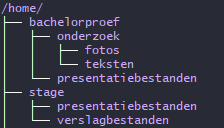
\includegraphics[width=0.45\textwidth]{img/mappenstructuur.png}}
	\caption{Mappen structuur basis configuraties.}
	\label{fig:mappen}
\end{figure}
\subsection{Opstellen cloud-init config bestand}
Als eerste zal het cloudconfig bestanden worden opgesteld. Dit bestand werd opgesteld met behulp van \autocite{clouddocs}.

Eerst werd er bekeken welke modules er nodig zullen zijn voor het opstellen van dit bestand. De modules \textit{packages} en \textit{package\_upgrade} zullen worden gebruikt voor de packages. De modules \textit{users} en \textit{groups} zullen worden gebruikt voor het toevoegen van gebruikers en groepen. 

Voor het toevoegen van de ssh sleutel, wordt de module \textit{ssh\_authorized\_keys} gebruikt. Hier worden de publieke sleutels die zijn toegelaten toegevoegd.

Voor het aanmaken van bestanden bestaat er de module \textit{write\_files}, spijtig genoeg is er geen module voor het aanmaken van mappen. Voor het aanmaken van de mappenstructuur werd dus de module \textit{runcmd} gebruikt.

\subsubsection{Packages}
Hierna werd het effectieve bestand gevormd. Onder de \textit{packages} werden de 3 packages opgelijst: \textit{git}, \textit{pwgen} en \textit{tree}. Bij \textit{package\_upgrade} werd \textit{true} gezet. 
\begin{lstlisting}[basicstyle=\small]
packages:
- pwgen
- git
- tree

package_upgrade: true
\end{lstlisting}

\subsubsection{Users \& Groups}
Bij \textit{groups} moest niet veel gedaan worden. Er werd gewoon de groepsnaam van de groep gezet.

Bij \textit{users} werden verschillende dingen ingevuld. Eerst en vooral de name, \textit{bachelor}. Bij groups de naam van de aangemaakte groep. Het wachtwoord onder passwd, proef, werd geëncrypteerd met de tool: \autocite{toolmkpass}. Als shell werd ook voor \textit{/bin/bash} gekozen.
\begin{lstlisting}[basicstyle=\small]
groups:
- test

users:
- default
- name: bachelor
- passwd: 985b56433efe9898290b88d4dab853a2f09d7eb7a7b1b8d2cdd431
- groups: test
- shell: /bin/bash
\end{lstlisting}


\subsubsection{Runcdm}
Bij de module \textit{runcmd} werden alle commando's gezet voor het aanmaken van de mappen structuur. Dit zijn gewoon 5 \textit{mdkir} commando's. Dit is het commando voor het aanmaken van mappen. Met de paramater \textit{-f} wordt heel de mappen structuur die meegegeven is, aangemaakt als die er nog niet is.
\begin{lstlisting}[basicstyle=\small]
runcmd:
- mkdir /home/bachelorproef/onderzoek/fotos -f
- mkdir /home/bachelorproef/onderzoek/teksten -f
- mkdir /home/bachelorproef/presentatiebestanden -f
- mkdir /home/stage/presentatiebestanden -f
- mkdir /home/stage/veslagbestanden -f
\end{lstlisting}

\subsubsection{Ssh}
Als laatste wordt de ssh sleutel toegevoegd aan de server. Bij de waarde \textit{<insert key value>} wordt de publieke sleutel van de host die gaat connecteren gezet.
\begin{lstlisting}[basicstyle=\small]
ssh_authorized_keys:
- ssh-rsa <INSERT KEY VALUE>
\end{lstlisting}

Helemaal onderaan werd ook iets gezet onder de module \textit{final\_message}, namelijk: \textit{"The system is finally up, after \$UPTIME seconds"}. Door de waarde \textit{\$UPTIME} kan er gekeken worden hoelang de server nodig had om alles uit te voeren.

\subsection{Opstellen Ansible playbook}
Als tweede werd het Ansible playbook opgesteld. Als host wordt gekozen voor localhost. Aan het \textit{ansible.cfg} bestand werd ook nog de regel \textit{callback\_whitelist = profile\_tasks}. Zo kan er bekeken worden hoelang het draaien van het playbook duurde. Alle configuraties die worden gedaan worden in verschillende \textit{tasks} gezet. 

\subsubsection{Packages}
Voor het upgraden van de packages en installeren van de nodige packages werd de task \textit{apt} gebruikt.
\begin{lstlisting}[basicstyle=\small]
- name: Upgrade all packages to the latest version
apt:
name: "*"
state: latest
- name: Install git
apt:
name: git
state: present
- name: Install tree
apt:
name: tree
state: present
- name: Install pwgen
apt:
name: pwgen
state: present
\end{lstlisting}
\subsubsection{Mappen structuur}
Voor het aanmaken van de mappen structuur werd de task \textit{file} gebruikt. De state werd dan op directory gezet.
\begin{lstlisting}[basicstyle=\small]
- name: Creates direcory fotos
file:
path: /home/bachelorproef/onderzoek/fotos
state: directory
- name: Creates direcory teksten
file:
path: /home/bachelorproef/onderzoek/teksten
state: directory
- name: Creates direcory bachelor presentatie
file:
path: /home/bachelorproef/presentatiebestanden
state: directory
- name: Creates direcory stage presentatie
file:
path: /home/stage/presentatiebestanden
state: directory
- name: Creates direcory stage verslag
file:
path: /home/stage/verslagbestanden
state: directory
\end{lstlisting}
\subsubsection{Users \& groups}
Bij het aanmaken van de gebruikers en groepen werden de tasks \textit{group} en \textit{user} gebruikt. Bij de \textit{user} werden het shell en password meegeven. Ook de groups werden meegegeven.
\begin{lstlisting}[basicstyle=\small]
- name:  add group test
group:
name: test
state: present
- name:  add user bachelor
user:
name: bachelor
groups: test
shell: /bin/bash
password: 985b56433efe9898290b88d4dab853a2f09d7eb7a7b1b8d2cdd431e2920c35
\end{lstlisting}

\subsubsection{Ssh}
Voor het toevoegen van de ssh sleutel aan de server, zodat er een extra connectie kan worden gelegd, wordt de task \textit{authorized\_key} gebruikt. De user die wordt meegegeven is de bachelor user.
\begin{lstlisting}[basicstyle=\small]
- name: Set authorized key taken from file
authorized_key:
user: bachelor
state: present
key: ssh-rsa <INSERT KEY VALUE>

\end{lstlisting}

\subsection{Ansible \& cloud-init omgevingen}
Beide bestanden die apart gemaakt zijn, zijn vrij complexloos. Beide bestanden zijn vrij duidelijk. Wat als nadeel is voor het gebruik van een combinatie van Ansible en cloud-init. De enige uitvoering die complex is de bestanden is het aanmaken van de mappen via cloud-init. Dit is een beetje 'dirty' gedaan. Voor het werken met een combinatie gaat eerst alles via cloud-init worden gedaan. Het aanmaken van de mappen dan via Ansible.

\subsubsection{Verwijzing Ansible}
Voor de cloud setup wordt de verwijzing via github gedaan. Er wordt een git repository aangemaakt met het playbook in. Die wordt dan gecloned in cloud-init en uitgevoerd.

In cloud-init wordt drie modules toegevoegd: \textit{runcmd} en \textit{ssh\_keys}. In de module \textit{ssh\_keys} wordt de private sleutel toegevoegd connectie legt met de git repo. In de module \textit{runcmd} worden 3 commando's gezet: het toevoegen van github aan het known host bestand, de git clone en het uitvoeren van het playbook. Bij de packages wordt ook de package \textit{ansible} gezet.
\begin{lstlisting}[basicstyle=\small]
ssh_keys:
rsa_private: | <key>
runcmd:
- ssh-keyscan github.com >> /etc/ssh/ssh_known_hosts
- ssh-agent bash -c 'ssh-add /etc/ssh/ssh\_host\_rsa\_key; 
git clone <repo>'
- ansible-playbook -i, /home/ansible/playbook.yaml
\end{lstlisting}


\section{Uitvoering \& resultaten}
\subsection{Complexiteit}
\subsubsection{Overzichtelijkheid}
Eerst en vooral wordt er gekeken naar het de overzichtelijkheid van het playbook bestand en het cloudconfig bestand. Terwijl beide bestanden yaml bestanden zijn, zien ze er toch compleet anders uit. In het cloudconfig bestand is alles mooi onderverdeeld in verschillende modules, die de taken uitvoert. Terwijl bij het Ansible playbook alles opgesomd bij de tasks staat. Cloud-init is hierdoor veel overzichtelijker. Het is hierdoor ook makkelijker om het bestand te wijzigen. Bij het gebruik van de combinatie het playbook wel overzichtelijker doordat dit maar een paar taken heeft. In figuur \ref{fig:basisconf_layout} staan de layouts van het cloud-init en Ansibles bestand.
\begin{figure}[!htb]
    \centering
    {{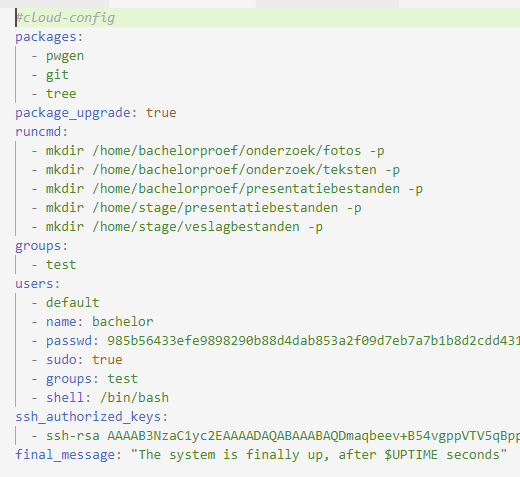
\includegraphics[width=0.45\textwidth]{img/basiscloud.png} }}%
    \qquad
    {{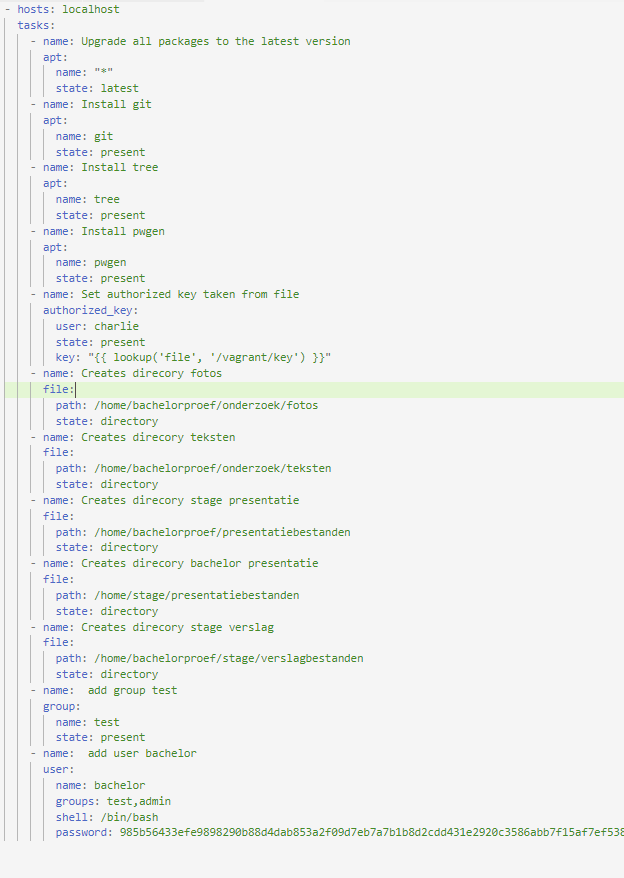
\includegraphics[width=0.45\textwidth]{img/basisansible.png} }}%
    \caption{Cloud-init en Ansible basis configuraties layout.}%
    \label{fig:basisconf_layout}%
\end{figure}
\subsubsection{Aanroepen uitvoeringen}
Ten tweede wordt er gekeken hoe alles werd aangeroepen. Voor het toevoegen van users, groepen en packages en het aanmaken van een nieuwe ssh sleutel zijn er voor Ansible en cloud-init aparte modules om dit te doen. Hier is weinig verschil. Maar voor het aanmaken van de mappen was er een verschil. Bij het toevoegen van de mappen is er bij Ansible een aparte module hiervoor. Terwijl bij cloud-init dit moest worden gedaan via runcmd en het \textit{mkdir} commando. 

Het aanroepen van de Ansible configuraties via cloud-init gebeurde via de commando module (\textit{runcmd}) in cloud-init. Dit gebeurde op een vrij efficiënte manier. Al moet er wel elke keer een private sleutel van de repo worden meegegeven.

\subsection{Snelheid}
Als er puur naar de snelheid wordt gekeken is Ansible duidelijk sneller. Maar cloud-init heeft configuraties die het altijd uitvoert. Hierdoor kan deze statistiek soms misleidend. De gemiddelde uitvoersnelheid voor Ansible is 137.53 seconden en voor cloud-init is dit 177.77 seconden. Als er bij cloud-init het verschil van de startup configuraties wordt afgetrokken, komt dit eerder op 140-145 seconden. Dit ligt veel dichter bij Ansible, dit verschil is eigenlijk verwerpbaar. Al is Ansible een beetje sneller is dit niet zo een groot verschil dat dit een voordeel is voor Ansible. Er kan worden vastgesteld dat ze min of meer dezelfde uitvoeringssnelheid hebben.

De cloud-init en Ansible configuraties hebben bijna dezelfde gemiddelde uitvoersnelheid als cloud-init, namelijk 177.60 seconden. Net zoals bij cloud-init kan er hier worden afgerond naar 140-145 seconden door de eerste basisconfiguraties van cloud-init. Ook hier is dus weer geen groot verschil merkbaar.

In tabel \ref{tab:tabel resultaten basis} staan de resultaten van de snelheden.

\begin{table}[!htb]
    \centering
    \begin{tabular}{| l | l | l |l |}
        \hline
        \textbf{Uitvoeringstijd} & Resultaat 1 & Resultaat 2 & Resultaat 3   \\ \hline
        cloud-init & 179.75 sec & 187.74 sec & 165.51 sec  \\ \hline
        Anisble & 168.69 sec & 132.59 sec & 111.31 sec \\ \hline
        cloud-init \& Ansible & 149.10 sec & 190.13 sec & 193.59 sec \\
        \hline
    \end{tabular}
    \caption{Snelheid van Basisconfiguraties op de servers.}
    \label{tab:tabel resultaten basis}
\end{table}

\subsection{Resultaat}
Voor basisconfiguraties lijkt het meteen wel beter om dit niet met Ansible en cloud-init te doen. Dit lijkt iets te omslachtig voor het maar basis werk dat moet gebeuren. 

Voor Ansible en cloud-init apart is er niet zoveel verschil. Terwijl het cloudconfig bestand wel veel overzichtelijker is, heeft Ansible iets meer variatie qua modules. Toch lijkt cloud-init in deze setup de beste optie. Het meegeven van het script gebeurt op een veel makkelijker manier. En doordat het maar basisconfiguraties zijn die hier worden getest, is het voordeel van de meer variatie van modules in Ansible nog niet zo doorslaggevend. De overzichtelijkheid van cloud-init is dat dan wel. Het bestand is veel compacter en veel duidelijker. Ook doordat het bestand op een makkelijkere manier kan worden uitgevoerd lijkt cloud-init hier de betere optie. Ansible geeft wel een betere output weer. Maar dit is hier nog niet doorslaggevend doordat er nog geen geavanceerde acties gebeuren.

Cloud-init lijkt, zeker als het in een gelijkaardige setup als deze gebeurt, de beste optie om eerste basisconfiguraties aan de server toe te voegen.

\chapter{\IfLanguageName{dutch}{Server installatie en configuratie}{Introduction}}
\label{ch:serverconf}
Dit hoofdstuk voert een tweede onderzoek. Er wordt gekeken hoe makkelijk een volledig type server wordt geïnstalleerd en geïmplementeerd. 

De twee type servers die worden geïnstalleerd zijn: MySQL en LAMP.

\section{LAMP server}
Een LAMP server is een van de populairste variaties van een webserver op linux. Via de documentatie van \autocite{lamp} wordt een kleine uitleg gegeven.

De 'L' staat voor Linux het besturingssysteem dat op de server draait. 

De 'A' staat voor apache dit is de web server software. 

De 'M' kan voor 2 dingen staan: MariaDB of MySQL. Dit zijn de database server softwares die worden gebruikt. In deze setup wordt gekozen voor MariaDB aangezien er al een aparte MySQL server wordt aangemaakt.

De 'P' staat voor PHP. Dit is de programmeer taal die de websites zullen gebruiken.

Een variatie op LAMP is LEMP. Dit is bijna hetzelfde alleen gebruikt het nginx als web server software in plaats van apache.


\subsection{Cloud-init}
Het bestand werd opgemaakt met behulp van \autocite{butcher}. Hierdoor krijgen we een basis lamp stack.

Allereerst werd het cloud-init script opgemaakt. Het script bevat niet zoveel functies. Het bevat 3 modules: \textit{package\_upgrade}(voor het updaten van de server packages), \textit{packages} (voor de packages die nodig zijn) en \textit{runcmd} (voor de taken die moeten worden uitgevoerd).

\subsubsection{Opmaken bestand}
\textit{Package\_upgrade} wordt allereerst op true gezet. Bij de \textit{packages} wordt: \textit{apache2, mysql-server, libapache2-mod-php5} en \textit{php5-mysql} gezet. Dit zijn de packages dit nodig zijn voor de lamp stack.
\begin{lstlisting}[basicstyle=\small]
package_upgrade: true

packages:
- apache2
- mysql-server
- libapache2-mod-php5
- php5-mysql
\end{lstlisting}

Bij \textit{runcmd} werden 2 commando's geplaats. Het eerste maakt het php bestand aan dat de server gaat gebruiken. Het tweede verwijdert het standaard html bestand.
\begin{lstlisting}[basicstyle=\small]
runcmd:
- echo '<?php phpinfo();' > /var/www/html/index.php
- rm /var/www/html/index.html
\end{lstlisting}


\subsection{Ansible}
Dit bestand werd opgemaakt met behulp van \autocite{bekker}. Dit maakt een basis lamp stack aan. Het playbook is onderverdeeld in 3 delen: installeren van de packages, starten van de services en het  toevoegen van het php bestand.

\subsubsection{Installeren packages}
Eerst en vooral worden de packages geïnstalleerd: \textit{apache2, my-sqlserver, php} en \textit{php-mysql}.
\begin{lstlisting}[basicstyle=\small]
- name: install lamp stack
become: yes
become_user: root
apt:
pkg:
- apache2
- mysql-server
- php
- php-mysql
state: present
update_cache: yes
\end{lstlisting}

\subsubsection{Starten services}
Als tweede werden de \textit{apache2} en \textit{mysql} server gestart. 
\begin{lstlisting}[basicstyle=\small]
- name: start apache service
become: yes
become_user: root
service:
name: apache2
state: started
enabled: yes

- name: start mysql service
become: yes
become_user: root
service:
name: mysql
state: started
enabled: yes
\end{lstlisting}

\subsubsection{Php bestand}
Ten laatste werd het php bestand aangemaakt en de map waar het moet komen. Het bestand kon via Ansible wel niet worden aangemaakt. Dus werd het via github meegeven. Het stond ook in de repo van het playbook.
\begin{lstlisting}[basicstyle=\small]
- name: create target directory
file: path=/var/www/html state=directory mode=0755

- name: deploy index.php
become: yes
become_user: root
copy:
src: /repo/index.hphp
dest: /var/www/html/index.php
\end{lstlisting}

\newpage
\subsection{Cloud-init \& Ansible}
\label{ch:cloudansiserverconf}
Voor de configuratie van Ansible en cloud-init worden de taken in 2 verdeeld. 

De packages worden geinstalleerd via cloud-init. Ook het aanmaken van het php bestand gebeurt via cloud-init. Het starten van de services wordt gedaan door Ansible ook het aanmaken van de directory wordt gedaan door Ansible.

\section{MySQL server}
De tweede server die werd gekozen is een MySQL server. MySQL is een database management systeem (DBMS). Een MySQL server is dus simpel weg een database server.

\subsection{Cloud-init}
Dit bestand werd opgemakt met behulp van \autocite{dias}.

Voorr het aanmaken van een MySQL server werden 3(4) modules gebruikt. Allereest de \textit{packages} (en \textit{package\_upgrade}) voor de packages, \textit{users} voor de database user en \textit{runcmd} voor de taken/commando's.

\subsubsection{Packages}
De packages die werden geïnstalleerd zijn: \textit{mysql-client, libmysqclient-dev} en \textit{mysql-server}.
\begin{lstlisting}[basicstyle=\small]
packages:
- mysql-client
- libmysqlclient-dev
- mysql-server

package_upgrade: true
\end{lstlisting}

\subsubsection{User}
Er werd een gebruiker toegevoegd dev. Met een ssh sleutel zodat er toegang is via deze gebruiker.
\begin{lstlisting}[basicstyle=\small]
users:
- name: dev
ssh-authorized-keys:
- ssh-rsa <key>
sudo: ['ALL=(ALL) NOPASSWD:ALL']
groups: sudo
shell: /bin/bash
\end{lstlisting}

\subsubsection{Commando's}
Ten laatste al de commando's die worden uitgevoerd. Hier wordt de mysql server geconfigureerd.
\begin{lstlisting}[basicstyle=\small]
runcmd:
- sed -i -e '/^Port/s/^.*$/Port 22/' /etc/ssh/sshd_config
- sed -i -e '/^PermitRootLogin/s/^.*$/PermitRootLogin no/' /etc/ssh/sshd_config
- sed -i -e '/^PasswordAuthentication/s/^.*$/PasswordAuthentication no/' /etc/ssh/sshd_config
- sed -i -e '$aAllowUsers dev' /etc/ssh/sshd_config
- sudo service ssh restart
- sudo ufw default deny incoming
- sudo ufw default allow outgoing
- sudo ufw allow ssh
- sudo ufw allow http
- sudo ufw allow https
- sed -i -e '/^ENABLED/s/^.*$/ENABLED=yes/' /etc/ufw/ufw.conf
- sudo ufw enable
\end{lstlisting}


\subsection{Ansible}
Dit bestand werd gemaakt met behulp van \autocite{hassin}.

Allereest werden weer de my-sql packages geïnstalleerd.
\begin{lstlisting}[basicstyle=\small]
- name: install my-sql
become: yes
become_user: root
apt:
pkg:
- mysql-server-core-5.7
- mysql-client-core-5.7
- libmysqlclient-dev
- python-mysqldb
- mysql-server
- mysql-client
\end{lstlisting}

Hierna werden de my-sql configuraties gedaan: het starten van de service, verwijderen van de test database, een my-sql gebruiker aanmaken, anonieme gebruikers verwijderen en het wachtwoord aanpassen voor de root gebruiker.
\begin{lstlisting}[basicstyle=\small]
- name: Start the MySQL service
action: service name=mysql state=started

- name: Remove the test database
mysql_db: name=test state=absent

- name: Create deploy user for mysql
mysql_user: user="deploy" host="%" password=maarten priv=*.*:ALL,GRANT

- name: Ensure anonymous users are not in the database
mysql_user: user='' host=localhost state=absent
with_items:
- 127.0.0.1
- ::1
- localhost

- name: Update mysql root password for all root accounts
mysql_user: name=root host=localhost password=maarten
with_items:
- 127.0.0.1
- ::1
- localhost
\end{lstlisting}


\subsection{Cloud-init \& Ansible}
Voor de configuratie van cloud-init en Ansible werden gelijkaardige dingen gedaan als bij LAMP. In principe werden bijna alle configuraties weer gedaan door Ansible. Alleen werden de packages geïnstalleerd door cloud-init.

\section{Uitvoering \& resultaten}
\subsection{Complexiteit}
Allereerst wordt de complexiteit weer bekeken. Daarin is er een verschil tussen MySQL en LAMP.

Bij de LAMP server is door de weinige configuraties, het cloud-init bestand heel overzichtelijk. Maar bij de MySQL server is dit dan weer niet. Doordat er verschillende configuraties worden gedaan en deze allemaal in de \textit{runcmd} module worden gedaan, is het bestand niet zo duidelijk. 

Bij Ansible daarentegen zijn er door de verschillende modules allemaal verschillende taken hiervoor apart. In deze setup zijn die verschillende taken wel overzichtelijk. 

Ook kunnen er met Ansible meer geavanceerde configuraties worden uitgevoerd bij beide servers. Cloud-init is beperkt tot de configuraties die via een commando kunnen worden gedaan. Ansible kan veel meer uitvoeren. 

\newpage
\subsection{Snelheid}
Qua snelheden is het vrij duidelijk. Ansible is veel efficiënter en sneller in het uitvoeren van de taken dan ``Ansible en cloud-init'' en cloud-init. Het verschil zonder de initiële configuraties doet er zelf niet toe. 

Dit is, t.o.v het vorige hoofdstuk, wel een verschil dat merkbaar is. Waardoor Ansible in dit onderdeel duidelijk de beter is ten opzichte van de andere 2 opties.

Ook is t.o.v. het vorige hoofdstuk het verschil tussen cloud-init en ``Ansible en cloud-init'' veel groter.

\begin{table}[!htb]
    \centering
    \begin{tabular}{| l | l | l |l |}
        \hline
        \textbf{Uitvoeringstijd} & Resultaat 1 & Resultaat 2 & Resultaat 3   \\ \hline
        cloud-init & 230.57 sec & 229.85 sec & 234.71 sec  \\ \hline
        Anisble & 62.71 sec & 76.10 sec & 65.48 sec \\ \hline
        cloud-init \& Ansible & 150.97 sec & 127.93 sec & 129.80 sec \\
        \hline
    \end{tabular}
    \caption{Snelheid tabel van LAMP configuraties op de servers.}
    \label{tab:tabel lamp resultaten server}
\end{table}

\begin{table}[!htb]
    \centering
    \begin{tabular}{| l | l | l |l |}
        \hline
        \textbf{Uitvoeringstijd} & Resultaat 1 & Resultaat 2 & Resultaat 3   \\ \hline
        cloud-init & 204.03 sec & 214.15 sec & 281.82 sec  \\ \hline
        Anisble & 29.26 sec & 35.86 sec & 111.31 sec \\ \hline
        cloud-init \& Ansible & 127.71 sec & 85.43 sec & 66.81 sec \\
        \hline
    \end{tabular}
    \caption{Snelheid tabel van MySQL configuraties op de servers.}
    \label{tab:tabel mysql resultaten server}
\end{table}

\subsection{Resultaat}
Voor server configuratie is het duidelijk dat Ansible de beste optie is. Ansible is veel sneller, overzichtelijker en heeft veel meer opties om te configureren. 

Ook door de output die Ansible geeft (Figuur \ref{fig:Ansibleoutput}) is het veel makkelijker om fouten uit een server configuratie te halen. Door de vele configuratie die deze scripts soms hebben, is het overzichtelijk dat in de output alles is opgelijst als 1 taak.
\begin{figure}[!htb]
    \center{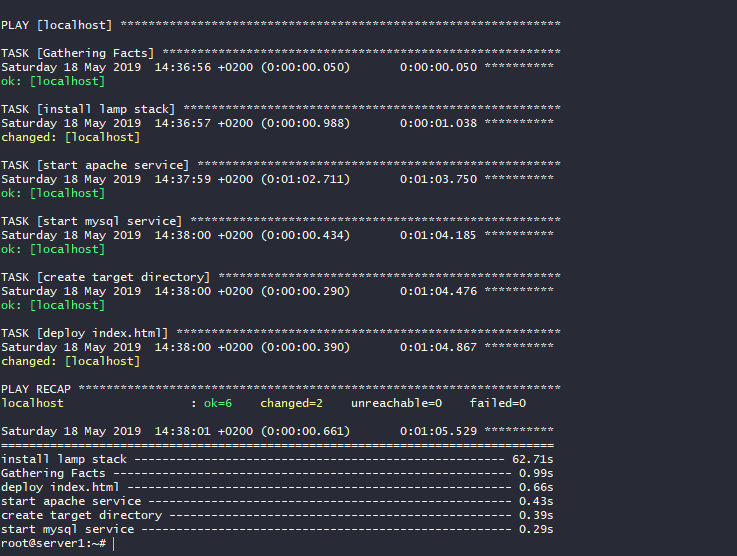
\includegraphics[width=1\textwidth]{img/ansibleoutput.png}}
    \caption{Ansible output voorbeeld.}
    \label{fig:Ansibleoutput}
\end{figure}

Al is cloud-init niet helemaal nutteloos hier. Als er bij de opstart van de server deze configuraties moeten worden gedaan. Is het de beste optie om cloud-init en Ansible te gebruiken. Doordat het cloud-init veel makkelijker kan worden meegegeven als een variabele. In dit script wordt er dan verwezen naar het Ansible playbook.

\chapter{\IfLanguageName{dutch}{Instellingen aanpassen na het opstarten}{Introduction}}
\label{ch:naopstarten}
In dit hoofdstuk wordt bekeken hoe makkelijk of moeilijk configuraties kunnen worden aangepast na het opstarten. Deze aanpassingen moeten dan wel gebeuren via Ansible en/of cloud-init.


\chapter{\IfLanguageName{dutch}{Container \& Cluster Configuratie}{Introduction}}
\label{ch:container}

HOOFDSTUK PAS MEERDERE SERVERS 

%%=============================================================================
%% Conclusie
%%=============================================================================

\chapter{Conclusie}
\label{ch:conclusie}

% TODO: Trek een duidelijke conclusie, in de vorm van een antwoord op de
% onderzoeksvra(a)g(en). Wat was jouw bijdrage aan het onderzoeksdomein en
% hoe biedt dit meerwaarde aan het vakgebied/doelgroep? 
% Reflecteer kritisch over het resultaat. In Engelse teksten wordt deze sectie
% ``Discussion'' genoemd. Had je deze uitkomst verwacht? Zijn er zaken die nog
% niet duidelijk zijn?
% Heeft het onderzoek geleid tot nieuwe vragen die uitnodigen tot verder 
%onderzoek?

Doorheen de bachelorproef werd er gezocht naar een antwoord op de vragen. Kunnen Ansible en cloud-init samen functioneren, zo ja hoe ? Maakt cloud-init Ansible overbodig? Na een onderzoek kan er antwoord gegeven worden op die vragen. 

Het resultaat wordt hierna vergeleken met de verwachte resultaten. 

Ten laatste wordt er besproken hoe dit onderzoek kan worden uitgebreid in de toekomst. Zijn er bijkomende vragen ontstaan?

\section{Antwoord op onderzoeksvragen}
Maakt cloud-init Ansible overbodig? Nee, eigenlijk niet. In de hoofdstukken \ref{ch:serverconf} en \ref{ch:container} werd gezien dat cloud-init, voor de meer geavanceerde configuratie, toch niet de juiste oplossing is. Als er servers moesten geconfigureerd worden met meerdere rules, schoot cloud-init nog te kort. De enige module waarin in kon gewerkt hiervoor was \textit{runcmd}. Ook werd in hoofdstuk \ref{ch:naopstarten} gezien dat cloud-init geen optie heeft om wijzigingen door te voeren en het script een tweede keer te draaien. Alleszins niet in de setup die hier wordt gebruikt. Al kan cloud-init wel voor bepaalde dingen gebruikt worden. In hoofdstuk \ref{ch:basisconf} werd gezien dat voor basisconfiguraties cloud-init misschien wel beter is dan Ansible. Cloud-init maakt Ansible dus zeker niet overbodig. Hiervoor zijn de modules te gelimiteerd. Maar als er een omgeving moet worden opgezet met juist basis configuraties, is het misschien aangeraden om cloud-init hiervoor te gebruiken.

\newpage
Kunnen Ansible en cloud-init samen functioneren? Ja, dit kunnen ze zeker, maar of dit moet worden gedaan hangt af van de situatie. Het samenwerken van cloud-init zou eerder nuttig zijn voor als de server wordt aangemaakt, er meteen configuratie willen meegegeven worden. Als dit niet het geval is, is een samenwerking niet aan te raden. Ook is een samenwerking alleen van nut als de configuraties die worden gedaan meer zijn dan de basis. In hoofdstuk \ref{ch:basisconf} werd gezien dat cloud-init de basis configuraties nog alleen kan doen zonder de hulp van Ansible.

Hoe kunnen ze samen functioneren? In praktijk lijkt het best om deze samen te gebruiken met elk zijn bepaalde functies. Cloud-init is in deze setup zeer goed als initieel script, doordat dit zo makkelijk kan worden meegegeven. In dit script kunnen eerste basis configuraties worden gedaan. Hierna wordt het Ansible playbook aangeroepen met de meer geavanceerde functies.

Als er een pure vergelijking wordt gedaan tussen de beide tools, is Ansible toch de winnaar. Ansible heeft, zoals hier al meerdere keren is aangehaald, veel meer functionaliteiten dan cloud-init. Ook heeft Ansible een veel duidelijkere output (Figuur \ref{fig:outputs}). Bij cloud-init wordt veel info getoond als het script loopt, dit kan wat overweldigend zijn. Terwijl bij Ansible alles mooi is opgelijst in de verschillende taken. Ook is het hierdoor veel makkelijker om eventuele fouten uit een script te halen.
\begin{figure}[!htb]
    \centering
    {{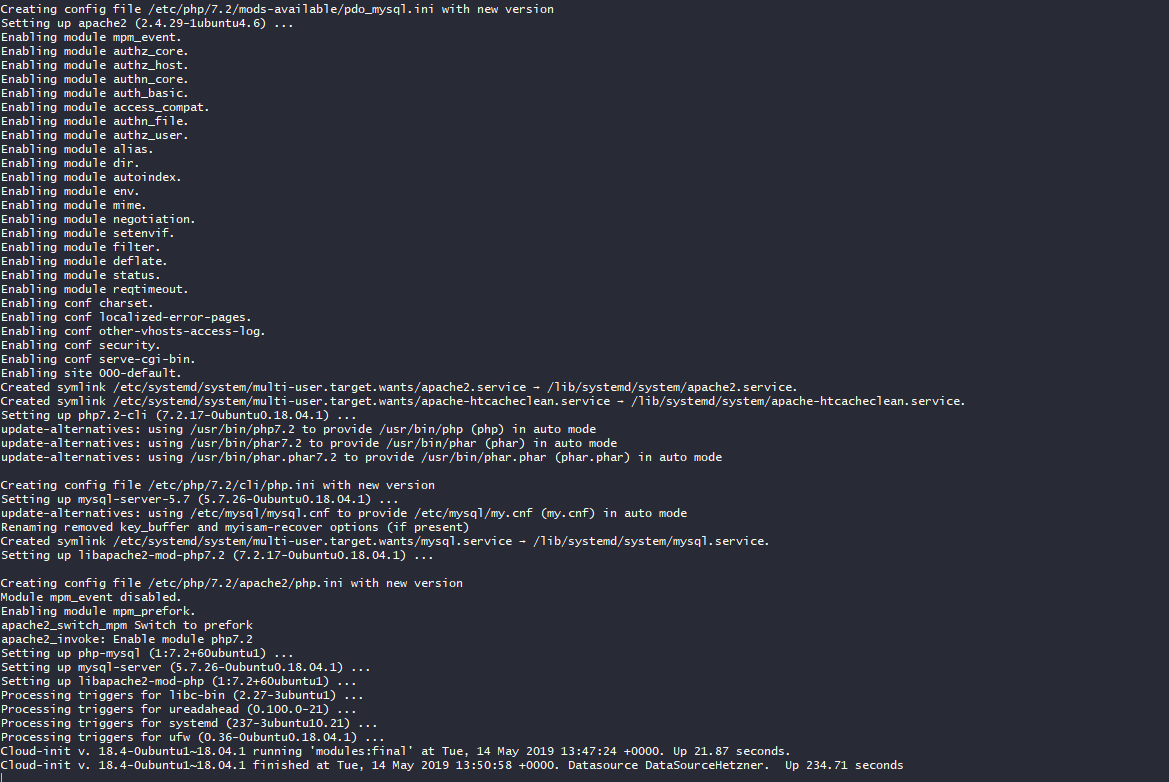
\includegraphics[width=0.45\textwidth]{img/cloudoutput.png} }}%
    \qquad
    {{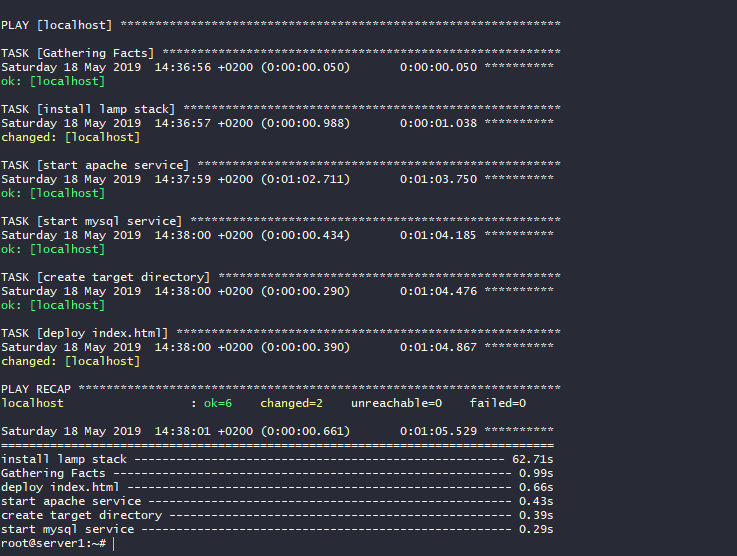
\includegraphics[width=0.45\textwidth]{img/ansibleoutput.png} }}%
    \caption{Cloud-init en Ansible outputs.}%
    \label{fig:outputs}%
\end{figure}

\section{Vergelijking met verwachte resultaten}
De verwachtingen zijn toch gedeeltelijke anders met de uiteindelijke resultaten/conclusies. In het voorstel werd er verwacht dat elke omgeving een ander oplossing ging hebben. Ook werd er verwacht dat de taken van Ansible en cloud-init gingen variëren van server tot server.

Dit is niet helemaal lijn met het effectieve resultaat. Er werd verwacht dat elke omgeving zijn eigen verhaal ging hebben en dat is toch niet gebeurt. Er kwam altijd één constante boven water. Cloud-init is goed voor de basis maar als er geavanceerder wilt gegaan worden is Ansible duidelijk beter. 

Uiteindelijk werd er verwacht dat cloud-init meer functionaliteiten ging hebben dan dat het uiteindelijk heeft. Er werd wel verwacht da Ansible ruimer ging zijn van mogelijkheden, aangezien dit veel populairder is. Maar er werd niet verwacht dat cloud-init er zoveel minder ging hebben.


\section{Verdere uitbreiding?}
Het onderzoek kan worden uitgebreid. Een restrictie die dit onderzoek had, is dat er maar met één cloud-provider kon worden gewerkt. Het zou interessant om te bekijken of er met andere providers hetzelfde resultaat zou hebben of niet. Ook de aanroeping van het cloud-init script en Ansible playbook kan op een andere manier. Door dit aan te aanroepen via een remote server. De servers worden dan opgesteld vanop een andere server en niet op de huidige server zoals hier. Weer zou het interessant zijn om te bekijken of een verandering invloed heeft op het resultaat.

De uiteindelijke vragen die na dit onderzoek kunnen worden gesteld zijn:
\begin{itemize}
    \item Hebben andere cloud-providers hetzelfde resultaat? 
    \item Heeft een andere aanroeping van de scripts een effect op het resultaat?
\end{itemize}



%%=============================================================================
%% Bijlagen
%%=============================================================================

\appendix
\renewcommand{\chaptername}{Appendix}

%%---------- Onderzoeksvoorstel -----------------------------------------------

\chapter{Onderzoeksvoorstel}

Het onderwerp van deze bachelorproef is gebaseerd op een onderzoeksvoorstel dat vooraf werd beoordeeld door de promotor. Dat voorstel is opgenomen in deze bijlage.

% Verwijzing naar het bestand met de inhoud van het onderzoeksvoorstel
%---------- Inleiding ---------------------------------------------------------

\section{Introductie} % The \section*{} command stops section numbering
\label{sec:introductie}

Voor de installatie van servers wordt al jaren Ansible gebruikt. Ansible is een universele 'taal' die taken voor servers automatiseert door middel van hun playbook. Zo een Ansible playbook is een georganiseerde unie van scripts dat het werk voor de server configuratie definieert.

Cloud-Init is momenteel een van de industrie standaarden voor het opbouwen van cloud servers, het maakt gebruik van cloud images. Dat zijn besturingssysteem sjablonen en elke instantie begint als een identieke kloon van elke andere instantie. De gebruikersgegevens geven elke cloud instantie haar persoonlijkheid. Doormiddel van cloud-int worden deze gegevens op de instantie toegepast. 

Dit zijn allebei provisioning systemen. Op een verschillende manier doen ze in theorie hetzelfde. Ze brengen de server allebei naar de gewenste toestand van de gebruiker. Doordat deze op verschillende manieren werken, wordt er in de praktijk in combinatie met beide gewerkt. In dat geval gebruik je eerste cloud-init om de server naar een gewenste toestand te brengen waar na Ansible het kan overnemen.

Maar is dit de perfecte samenwerking? Het bedrijf Be-mobile is opzoek naar het antwoord. In dit onderzoek bestuderen we waar deze mekaar aanvullen en hoe ze dan op een perfect performante manier werken. Natuurlijk is het goed mogelijk dat deze mekaar niet aanvullen en dan is het onderzoek waar en wanneer je voor wat moet kiezen en waarom dit mekaar overbodig maakt. 

In dit onderzoek zullen we dit trachten te ontdekken. De vragen waar het, de antwoorden op wil vinden zijn:
\begin{itemize}
	\item Vullen Ansible en Cloud-Init mekaar aan, of maken ze elkaar overbodig?
	\item Ook hoe ze mekaar aanvullen en/of hoe ze mekaar overbodig maken?
\end{itemize}

%Hier introduceer je werk. Je hoeft hier nog niet te technisch te gaan.

%Je beschrijft zeker:

%\begin{itemize}
%  \item de probleemstelling en context
%  \item de motivatie en relevantie voor het onderzoek
%  \item de doelstelling en onderzoeksvraag/-vragen
%\end{itemize}

%---------- Stand van zaken ---------------------------------------------------

\section{Stand Van Zaken}
\label{sec:state-of-the-art}

Ansible en Cloud-Init zijn geen onbekende voor mekaar dus er is wel een basis gevonden waarop er verder kan gewerkt worden. Maar zijn niet zo bekend dat de ultieme samenwerking al gevonden is. In het onderzoeken van de 2 systemen zijn er 5 artikels gevonden die een samenwerking beschrijven of afraden. 


In de artikels \textbf{"An introduction to server provisioning with CloudInit"\autocite{Cloudsigma}}, \textbf{“Using Ansible to Bootstrap My Work Environment Part 4” \autocite{scottharney}} en \textbf{“Customizing Cloud Assembly Deployments with Cloud-Init” \autocite{vmware}} is er een vaak voorkomend fenomeen gevonden. Meestal gebruiken de gebruikers/auteurs eerst cloud-init om de machine op te starten, daarna ansible voor de verdere specifieke eigenschappen.


Het artikel geschreven door \textcite{Cloudsigma} is wel interessant doordat hij ook andere systemen buiten cloud-init heeft getest, waaronder puppet en chef. Maar toch verkiest hij om Ansible te gebruiken. Dit betekent dat een samenwerking met ansible optimaler is.


De artikels \textbf{“Zero Touch Provisioning of Infoblox Grid on OpenStack using Ansible”\autocite{infoblox}} en \textbf{"Automated Ansible AWX Installation" \autocite{deven}} beschrijven dan weer hoe beide elke als een apart systeem kunnen worden gebruikt zonder de hulp van de ander. Maar toch zijn er een paar gelijkenissen zo gebruikt \textcite{deven} in "Automated Ansible AWX Installation" notities van een Ansible installatie om het met cloud-init te installeren.


Er is duidelijk al bekend dat er samengewerkt kan worden, maar ook soms weer niet. Maar criteria om te bepalen wanneer welke het best is, is nog niet bekend. 








%Hier beschrijf je de \emph{state-of-the-art} rondom je gekozen onderzoeksdomein. Dit kan bijvoorbeeld een literatuurstudie zijn. Je mag de titel van deze sectie ook aanpassen (literatuurstudie, stand van zaken, enz.). Zijn er al gelijkaardige onderzoeken gevoerd? Wat concluderen ze? Wat is het verschil met jouw onderzoek? Wat is de relevantie met jouw onderzoek?

%Verwijs bij elke introductie van een term of bewering over het domein naar de vakliteratuur, bijvoorbeeld~\autocite{Doll1954}! Denk zeker goed na welke werken je refereert en waarom.

% Voor literatuurverwijzingen zijn er twee belangrijke commando's:
% \autocite{KEY} => (Auteur, jaartal) Gebruik dit als de naam van de auteur
%   geen onderdeel is van de zin.
% \textcite{KEY} => Auteur (jaartal)  Gebruik dit als de auteursnaam wel een
%   functie heeft in de zin (bv. ``Uit onderzoek door Doll & Hill (1954) bleek
%   ...'')


%---------- Methodologie ------------------------------------------------------
\section{Methodologie}
\label{sec:methodologie}

Dit onderzoek zal gevoerd worden door virtuele server omgevingen op te zetten met Cloud-init en/of Ansible. De programma’s die hierbij zullen worden gebruikt zijn VirtualBox, Vagrant en Atom. 

Virtualbox is een programma om virtuele machines op te draaien. Met Vagrant kan je van in je shell met een simpel commando virtuele machines op starten. Atom is dan weer een teksteditor om de configuratie goed in neer te pennen. Normaal is deze het vermelden niet waar maar door de overzichtelijke manier van werken die het aanbiedt is deze toch veel beter dan een gewone Notepad.

Met Ansible zal er voor verschillende servers een testomgeving worden opgezet. Dit zal dan ook gebeuren met cloud-init. Deze resultaten en omgevingen kunnen dan worden  vergeleken met elkaar. De technische eigenschappen/resultaten worden dan onder de loep genomen: de performantie, de snelheid van het opstarten,… Ook zal er worden gekeken naar de config files van beiden en kan er worden gekeken welke daar per omgeving “beter” is. M.a.w. welke er op een kortere overzichtelijkere manier hetgeen kan bekomen. Be-Mobile kan ook nog verdere criteria bepalen waardoor we een keuze gaan maken. Daarna worden ook  combinaties van de twee aangemaakt en dan kunnen we deze vergelijken met de originele servers. 

Ook kan het zijn dat er vragen worden gesteld aan medewerkers van het bedrijf Be-Mobile om te bekijken wat hun mening over beide is.

%Hier beschrijf je hoe je van plan bent het onderzoek te voeren. Welke onderzoekstechniek ga je toepassen om elk van je onderzoeksvragen te beantwoorden? Gebruik je hiervoor experimenten, vragenlijsten, simulaties? Je beschrijft ook al welke tools je denkt hiervoor te gebruiken of te ontwikkelen.

%---------- Verwachte resultaten ----------------------------------------------
\section{Verwachte resultaten}
\label{sec:verwachte_resultaten}
De verwachtingen zijn dat een combinatie van cloud-init en Ansible meestal het beste zal zijn. Dat er voor elke server tot een bepaald moment cloud-init of ansible  zal worden gebruikt waarna ansible of cloud-init het zal overnemen. Ook zijn de verwachtingen dat er voor elke omgeving een andere oplossing zal zijn. Er zal veel afhangen van het type besturingssysteem dat draait en van de servers om te kunnen bepalen welke het best wordt gekozen. 

De verwachtingen zijn ook dat niet bij alles een combinatie zal worden gebruikt. Ook kan het misschien zijn dat het beter is dat je één van beide kiest voor een bepaalde server omgeving.


%Hier beschrijf je welke resultaten je verwacht. Als je metingen en simulaties uitvoert, kan je hier al mock-ups maken van de grafieken samen met de verwachte conclusies. Benoem zeker al je assen en de stukken van de grafiek die je gaat gebruiken. Dit zorgt ervoor dat je concreet weet hoe je je data gaat moeten structureren.

%---------- Verwachte conclusies ----------------------------------------------
\section{Verwachte conclusies}
\label{sec:verwachte_conclusies}
De verwachte conclusie is dat elke server omgeving een andere uitkomst zal hebben. Er veel zal afhangen van welke server je precies wilt draaien op welk systeem. Dan kan er worden gekozen voor een bepaalde combinatie van beide of misschien één van beide. De conclusie zal niet zijn welke van de twee beter is. Maar eerder hoe ze het best gebruikt worden per serveromgeving.



%Hier beschrijf je wat je verwacht uit je onderzoek, met de motivatie waarom. Het is \textbf{niet} erg indien uit je onderzoek andere resultaten en conclusies vloeien dan dat je hier beschrijft: het is dan juist interessant om te onderzoeken waarom jouw hypothesen niet overeenkomen met de resultaten.



%%---------- Andere bijlagen --------------------------------------------------
% TODO: Voeg hier eventuele andere bijlagen toe
%\input{...}

%%---------- Referentielijst --------------------------------------------------

\printbibliography[heading=bibintoc]

\end{document}
